\subsection{Completing the Square Method for Quadratics}
\begin{definition}[Completing the Square]
	An algebraic method used to rewrite a quadratic expression from its standard form, $ax^2 + bx + c$, into the vertex form, $a(x - h)^2 + k$. This transformation creates a perfect square binomial.
\end{definition}
\begin{example}[Completing the square]
	\hfill
	\begin{enumerate}
		\item $f(x) = x^2 + 4x - 3$ \\
			$0 = x^2 + 4x - 3$ \\
			\textbf{Note: }We're gonna pretend $-3$ isn't there. \\
			$0 = x^3 - 4x \qquad - 3$ \\
			\begin{center}
				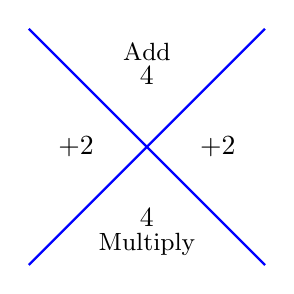
\begin{tikzpicture}[scale=1.5, auto, >=stealth]
					\draw[thick, blue] (-1, 1) -- (1, -1);
					\draw[thick, blue] (-1, -1) -- (1, 1);
					\node at (0, 0.6) {4};
					\node at (0, -0.6) {4};
					\node at (-0.6, 0) {+2};
					\node at (0.6, 0) {+2};
					\node at (0, 0.6) [above=2pt] {\small Add};
					\node at (0, -0.6) [below=2pt] {\small Multiply};
				\end{tikzpicture}
			\end{center}
			$0 = (x^2 + 4x + 4) -4 -3$ \qquad $(x + 2) (x + 2) = (x + 2)^2$ \\
			$0 = (x + 2)^2 - 7$ \\
			$(x + 2)^2 = 7$ \\
			$\sqrt{(x + 2)^2} = \pm \sqrt{7}$ \\
			$x + 2 = \pm \sqrt{7}$ \\
			$x = -2 \pm \sqrt{7}$ \\
			$x = -2 + \sqrt{7} \land x = -2 -\sqrt{7}$
		\item $g(x) = x^2 - 3x + 1$ \\
			$x^2 - 3x + 1 = 0$ \\
			$(x^2 - 3x \qquad) + 1 = 0$ \\
			\begin{center}
				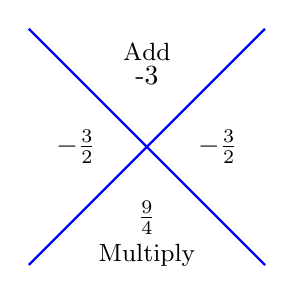
\begin{tikzpicture}[scale=1.5, auto, >=stealth]
					\draw[thick, blue] (-1, 1) -- (1, -1);
					\draw[thick, blue] (-1, -1) -- (1, 1);
					\node at (0, 0.6) {-3};
					\node at (0, -0.6) {$\frac{9}{4}$};
					\node at (-0.6, 0) {$-\frac{3}{2}$};
					\node at (0.6, 0) {$-\frac{3}{2}$};
					\node at (0, 0.6) [above=2pt] {\small Add};
					\node at (0, -0.6) [below=6pt] {\small Multiply};
				\end{tikzpicture}
			\end{center}
			$(x^2 - 3x + \frac{9}{4}) -\frac{9}{4} + 1 = 0$ \\
			$(x - \frac{3}{2})^2 - \frac{5}{4} = 0$ \\
			$(x - \frac{3}{2})^2 = \frac{5}{4}$ \\
			$\sqrt{(x - \frac{3}{2})^2} = \pm \sqrt{\frac{5}{4}}$ \\
			$x -\frac{3}{2} = \pm \frac{\sqrt{5}}{2}$ \\
			$x = \frac{3}{2} \pm \frac{\sqrt{5}}{2}$ \\
			$x = \frac{3 + \sqrt{5}}{2} \land x = \frac{3 - \sqrt{5}}{2}$
		\item $h(x) = 5x^2 - 10x + 2$ \\
			$5x^2 - 10x + 2 = 0$ \\
			$5(x^2 - 2x \qquad) + 2 = 0$ \\
			\begin{center}
				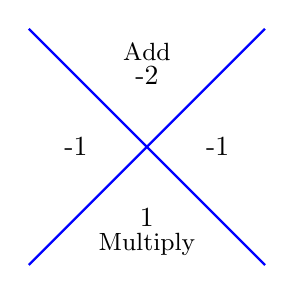
\begin{tikzpicture}[scale=1.5, auto, >=stealth]
					\draw[thick, blue] (-1, 1) -- (1, -1);
					\draw[thick, blue] (-1, -1) -- (1, 1);
					\node at (0, 0.6) {-2};
					\node at (0, -0.6) {1};
					\node at (-0.6, 0) {-1};
					\node at (0.6, 0) {-1};
					\node at (0, 0.6) [above=2pt] {\small Add};
					\node at (0, -0.6) [below=2pt] {\small Multiply};
				\end{tikzpicture}
			\end{center}
			\textbf{Note: }Remember to subtract $1$ by $5$ because its multiplied by $5$. \\
			$5(x^2 - 2x + 1) - 5 + 2 = 0$ \\
			$5(x - 1)^2 - 3 = 0$ \\
			$(x - 1)^2 = \frac{3}{5}$ \\
			$\sqrt{(x - 1)^2} = \pm \sqrt{\frac{3}{5}}$ \\
			$x = -1 \pm \sqrt{\frac{3}{5}}$ \\
			$x = -1 - \sqrt{\frac{3}{5}} \land x = -1 + \sqrt{\frac{3}{5}}$
		\item $g(x) = x^2 + \frac{2}{3}x - \frac{1}{3}$ \\
			$x^2 = \frac{2}{3}x - \frac{1}{3}$ \\
			$(x^2 + \frac{2}{3}x \qquad) - \frac{1}{3}$ \\
			\begin{center}
				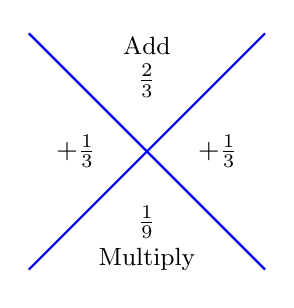
\begin{tikzpicture}[scale=1.5, auto, >=stealth]
					\draw[thick, blue] (-1, 1) -- (1, -1);
					\draw[thick, blue] (-1, -1) -- (1, 1);
					\node at (0, 0.6) {$\frac{2}{3}$};
					\node at (0, -0.6) {$\frac{1}{9}$};
					\node at (-0.6, 0) {$+\frac{1}{3}$};
					\node at (0.6, 0) {$+\frac{1}{3}$};
					\node at (0, 0.6) [above=6pt] {\small Add};
					\node at (0, -0.6) [below=6pt] {\small Multiply};
				\end{tikzpicture}
			\end{center}
			$(x^2 + \frac{2}{3}x + \frac{1}{9}) - \frac{1}{9} - \frac{1}{3} = 0$ \\
			$(x + \frac{1}{3})^2 - \frac{4}{9} = 0$ \\
			$(x + \frac{1}{3})^2 = \frac{4}{9}$ \\
			$\sqrt{(x + \frac{1}{3})^2} = \pm \sqrt{\frac{4}{9}}$ \\
			$x + \frac{1}{3} = \pm \frac{2}{3}$ \\
			$x = -\frac{1}{3} \pm \frac{2}{3}$ \\
			$x = -\frac{1}{3} - \frac{2}{3} \to \frac{1}{3} \land x = -\frac{1}{3} + \frac{2}{3} \to -1$
		\item $f(x) = 3x^2 + x - \frac{1}{2}$ \\
			$3x^2 + x - \frac{1}{2} = 0$ \\
			$3(x^2 + \frac{1}{3}x \qquad) -\frac{1}{2} = 0$ \\
			\begin{center}
				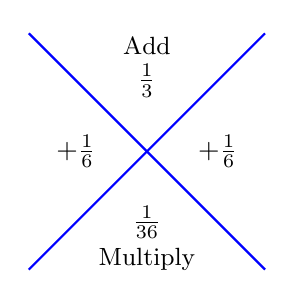
\begin{tikzpicture}[scale=1.5, auto, >=stealth]
					\draw[thick, blue] (-1, 1) -- (1, -1);
					\draw[thick, blue] (-1, -1) -- (1, 1);
					\node at (0, 0.6) {$\frac{1}{3}$};
					\node at (0, -0.6) {$\frac{1}{36}$};
					\node at (-0.6, 0) {$+\frac{1}{6}$};
					\node at (0.6, 0) {$+\frac{1}{6}$};
					\node at (0, 0.6) [above=6pt] {\small Add};
					\node at (0, -0.6) [below=6pt] {\small Multiply};
				\end{tikzpicture}
			\end{center}
			$3(x^2 + \frac{1}{3}x + \frac{1}{36}) - \frac{1}{12} -\frac{1}{2} = 0$ \\
			$3(x + \frac{1}{6})^2 - \frac{7}{12} = 0$ \\
			$3(x + \frac{1}{6})^2 = \frac{7}{12}$ \\
			$(x + \frac{1}{6})^2 = \frac{7}{36}$ \\
			$\sqrt{(x + \frac{1}{6})^2} = \pm \sqrt{\frac{7}{36}}$ \\
			$x + \frac{1}{6} = \pm \sqrt{\frac{7}{36}}$ \\
			$x = -\frac{1}{6} \pm \sqrt{\frac{7}{36}}$ \\
			$x = -\frac{1}{6} + \sqrt{\frac{7}{36}} \land x = -\frac{1}{6} - \sqrt{\frac{7}{36}}$
	\end{enumerate}
\end{example}
